%!TEX root = main.tex

\section{Funciones continuas sobre espacios métricos}

A lo largo de este capítulo se notará un uso recurrente de todo lo que se ha visto en el curso... diría que este capítulo es el que coneptualmente es más complejo por esto mismo, en este punto es necesario tener claros todos los conceptos para no perderse.

\begin{note}
Para este capítulo es importante saberse todas las propiedades que se presentan al inicio ya que serán usadas en muchas demostraciones posteriores,también es importante tener claras las definiciones equivalentes de continuidad...
\end{note}

\section{Quiz 10}



\begin{itemize}[label={✎},leftmargin=*]

\item Consideremos $(\mathbb{N},d_1)$ y $(E,d)$ espacio métrico. Si $f: \mathbb{N} \longrightarrow E$, entonces $f$ es continua.\\

\begin{proof}
 Note que todos los puntos en $(\mathbb{N},d_1)$ son aislados, puesto que, visto $\mathbb{N}$ como subespacio de $(\mathbb{R},d_1)$, dado $n \in \mathbb{N}$, podemos tomar $B(n;\frac{1}{2}) \cap \mathbb{N}=\{n\}$, por lo tanto, $f: \mathbb{N} \longrightarrow E$ es continua, ya que cualquier función entre espacios métricos es continua en puntos aislados
\end{proof}

\item Sean $(E_1,d_1)$, $(E_2,d_2)$ espacios métricos. Si $f: E_1 \longrightarrow E_2$ es continua, entonces $f$ envía conjuntos abiertos de $E_1$ en conjuntos abiertos de $E_2$.\\

Falso: Considere  $(E_1,d_1)=(E_2,d_2)=(\mathbb{R},d_1)$ y 
    \begin{align*}
        f: \hspace{2mm} &\mathbb{R} \longrightarrow \mathbb{R}\\
        &x \longmapsto 1 
    \end{align*}
    Esta función es continua, sin embargo, podemos tomar por ejemplo $A=(0,1)$ abierto de $(\mathbb{R},d_1)$, sin embargo, $f(A)=\{1\}$ que no es abierto en $(\mathbb{R},d_1)$

\item Sean $(E_1,d_1)$, $(E_2,d_2)$ espacios métricos. Si $f: E_1 \longrightarrow E_2$ es continua, entonces $f^{-1}(B)$ es cerrado en $E_1$ si $B$ es cerrado en $E_2$.\\

\begin{proof}
 Considere $B$ cerrado en $E_2$, luego, $B^c$ es abierto en $E_2$. Como $f$ es continua, entonces $f^{-1}(B^c)$ es abierto en $E_1$, además tenemos la relación $f^{-1}(B^c)=(f^{-1}(B))^c$ y por lo tanto, $f^{-1}(B)$ es cerrado en $E_1$.
\end{proof}

\item En $(\mathbb{R},d_1)$ la función
\begin{align*}
    \chi_\mathbb{Q}: \hspace{2mm} &\mathbb{R} \longrightarrow \mathbb{R}\\
    &x \longmapsto \begin{cases}
        1 & \text{si } x\in \mathbb{Q}\\
        0 & \text{si } x \notin \mathbb{Q}
    \end{cases}
\end{align*}
es continua.

Falso: Considere $A=(0,2)$ abierto en $(\mathbb{R},d_1)$. Tenemos que $\chi_{\mathbb{Q}}^{-1}(A)=\mathbb{Q}$ que no es abierto en $(\mathbb{R},d_1)$, luego $\chi_{\mathbb{Q}}$ no es continua.

\item Sean $(E_1,d_1)$, $(E_2,d_2)$ espacios métricos. Si $f: E_1 \longrightarrow E_2$ es continua, entonces $f$ envía conjuntos acotados de $E_1$ en conjuntos acotados de $E_2$.

Falso: Considere $(E_1,d_1)=(\mathbb{R}^+,d_1)$,$(E_2,d_2)=(\mathbb{R},d_1)$ y la función
    \begin{align*}
        f: \hspace{2mm} &\mathbb{R}^+ \longrightarrow \mathbb{R}\\
        &\hspace*{0.32cm}x \longmapsto ln(x)
    \end{align*}
Esta función es continua. Sea $A=(0,1)$ acotado en $(\mathbb{R}^+,d_1)$, sin embargo $f(A)=(-\infty,0)$ que es no acotado en $(\mathbb{R},d_1)$.

\end{itemize}

\section{Funciones entre espacios métricos compactos}

Este capítulo de las notas contiene ya uno de los acercamientos a lo que conocimos en cálculo diferencial, en particular el teorema del valor intermedio, aquí se puede intuir geométricamente la importancia de  la conexidad para este resultado y muchos más a lo largo del capítulo

\section{Quiz 11:}

\begin{itemize}[label={✎},leftmargin=*]

\item  Si $f:[a, b] \rightarrow \mathbb{R}$ tal que $f(x)=x^3$ entonces $f$ es uniformemente continua.\\

\begin{proof}
Note que $[a,b]$ es compacto porque es cerrado y acotado en $\R$, además $x^3$ es continua, por tanto $x^3$ es uniformemente continua en $[a,b]$.
\end{proof}

\item Si $f:(1,2) \rightarrow \mathbb{R}$ tal que $f(x)=x^3$ entonces $f$ es uniformemente continua\\

 \begin{proof}
 Sea $\varepsilon>0$, considere $\delta=\frac{\varepsilon}{12}$. Sean $x,y \in (1,2)$, note que si $|x-y|<\delta$:

 \begin{align*}
    |x^3-y^3|&=|x-y||x^2+xy+y^2|\\
    &<\delta|x^2+xy+y^2|\\
    &<\delta|4+4+4|\\
    &=\frac{\varepsilon}{12}(12)\\
    &=\varepsilon
 \end{align*}
 \end{proof}    


\item  Sean $\left(E_1, d_1\right),\left(E_2, d_2\right)$ espacios métricos y $f: E_1 \rightarrow E_2$ función continua. Si $K$ es compacto en $E_2$, entonces $f^{-1}(K)$ es compacto en $E_1$.

Falso: Considere:

\begin{align*}
    f: &\mathbb{R} \longrightarrow \mathbb{R}\\
&\hspace*{0.05cm}x \longmapsto 1
.\end{align*}

Claramente $f$ es continua y $\{1\}$ es compacto en $(\R,d_1)$, pero $f^{-1}(\{1\})=\R$, que no es compacto en $(\R,d_1)$

\item Sean $\left(E_1, d_1\right),\left(E_2, d_2\right)$ espacios métricos y $f: E_1 \rightarrow E_2$ función continua. Si $K$ es compacto en $E_1$, entonces $f(K)$ es cerrado y acotado en $E_2$.\\

\begin{proof}
En efecto como $f$ es continua y $K$ es compacto, $f(K)$ es compacto, por tanto es cerrado y acotado.
\end{proof}

\item  Sean $\left(E_1, d_1\right),\left(E_2, d_2\right)$ espacios métricos y $f: E_1 \rightarrow E_2$ función continua. Si $\left\{x_n\right\}_{n \in \mathbb{N}}$ es de Cauchy en $E_1$, entonces $\left\{f\left(x_n\right)\right\}_{n \in \mathbb{N}}$ es de Cauchy en $E_2$.

Falso: Sean $(E_1,d_1)=(E_2,d_2)=(\R^+,d_1)$, considere la sucesión de Cauchy $\{\frac{1}{n}\}_{n\in \N}$ y la función continua $f(x)=\frac{1}{x}$, note que $\{f(\frac{1}{n})\}_{n\in \N}=\{n\}_{n\in \N}$ que no es de cauchy porque no es acotada.

\item Sean $\left(E_1, d_1\right),\left(E_2, d_2\right)$ espacios métricos y $f: E_1 \rightarrow E_2$ función continua. Si $E_1$ es compacto $y\left\{x_n\right\}_{n \in \mathbb{N}}$ es de Cauchy en $E_1$, entonces $\left\{f\left(x_n\right)\right\}_{n \in \mathbb{N}}$ es convergente en $E_2$\\

\begin{proof}
Note que $E_1$ es compacto y por tanto completo, luego $\{x_n\}_{n\in\N}$ converge a $L \in E_1$, además:

$$\lim_{n\to \infty}f(x_n)=f\left(\lim_{n\to \infty} x_n\right)=f(L)$$

Por tanto $\{f(x_n)\}_{n\in \N}$ converge
\end{proof}

\item El conjunto $B(0,1) \backslash\{0\}$ es conexo en $\left(\mathbb{R}^n, d_2\right)$ para $n \geq 2$.\\




\begin{basedtikz}
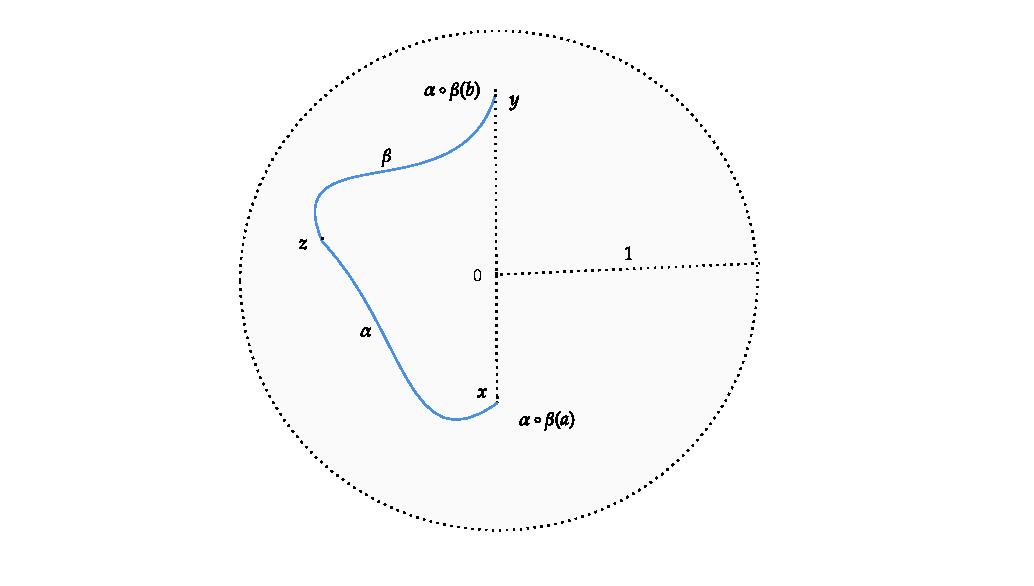
\includegraphics{{Graphics/conexidad}}
\end{basedtikz}



\begin{proof}
Tenemos que $B(0,1)$ es conexo en $(\R^n,d_2)$, luego como $B(0,1)$ es abierto, en particular es arcoconexo, veamos que $B(0,1)\setminus \{0\}$ es arcoconexo en $(\R^n,d_2)$.\\

Sean $x,y\in B(0,1)$, note que como $B(0,1)$ es arcoconexo, existe $z\in B(0,1)\setminus\{0\}$ tal que $\alpha: [a,b]\mapsto B(0,1)\setminus\{0\}$ tal que $\alpha(a)=x$ y $\alpha(b)=z$ y $\beta: [a,b]\mapsto B(0,1)\setminus\{0\}$ tal que $\alpha(a)=z$ y $\alpha(b)=y$, luego como composición de funciones continuas es continua $\alpha \circ \beta: [a,b]\mapsto B(0,1)\setminus \{0\}$ es un camino tal que $\alpha \circ \beta (a)=x$ y $\alpha \circ \beta(b)=y$, así $B(0,1)\setminus \{0\}$ es arcoconexo y por tanto conexo. 
\end{proof}

\item  Sean $\left(E_1, d_1\right),\left(E_2, d_2\right)$ espacios métricos y $f: E_1 \rightarrow E_2$ una función. Si $f$ envía conjuntos compactos en conjuntos compactos entonces $f$ es continua\\

Falso: Sean $(E_1,d_1)=(E_2,d_2)=(\R,d_1)$, considere la función:

\begin{align*}
    \chi_\mathbb{Q}: \hspace{2mm} &\mathbb{R} \longrightarrow \mathbb{R}\\
    &x \longmapsto \begin{cases}
        1 & \text{si } x\in \mathbb{Q}\\
        0 & \text{si } x \notin \mathbb{Q}
    \end{cases}
\end{align*}

Esta función mapea compactos en compactos ya que todo conjunto finito en $(\R,d_1)$ es compacto, en particular $\{0,1\},\{0\}$ y $\{1\}$, pero sabemos que $\chi_{\Q}$ no es continua.

\end{itemize}

\section{Homeomorfismos}

Intuitivamente podemos pensar que los homeomorfismos nos permiten ver cuando dos espacios métricos tienen las mismas propiedades topológicas, esto ocurre ya que en muchas de las propiedades que se vieron en la sección anterior se probó que si $f$ es continua entonces mapea compactos en compactos, devuelve abiertos en abiertos, también toda sucesión convergente la mapea a una sucesión convergente, mapea conexos en conexos, etc. Note que el homeomorfismo pide que $f$ sea biyectiva y que $f^{-1}$ sea continua también, es decir que la inversa también cumple todas las propiedades antes mencionadas, esto nos da una correspondencia explícita entre cada conjunto que cumple una de las propiedades mencionadas en el espacio de salida con uno en el de llegada y viceversa, por tanto preservan la información topológica que nos interesa en este contexto.

\section{Quiz 12}

\begin{itemize}[label={✎},leftmargin=*]
    \item Dados $r_1, r_2>0$ y $a, b \in \mathbb{R}^n$, existe $f: B\left(a, r_1\right) \rightarrow B\left[b, r_2\right]$ homeomorfismo.

Falso: Tome $(\R,d_1)$ y $r_1,r_2=1$ y $a,b=0$, entonces $[-1,1]$ es compacto, como $f^{-1}$ es continua y biyectiva, $f^{-1}([-1,1])=(-1,1)$, luego $(-1,1)$ es compacto como subespacio de $(\R,d_1)$, contradicción ya que $(-1,1)\cong \R$ y $\R$ no es compacto. 

\item Existe un homeomorfismo entre $\mathbb{R}^n$ y una bola cerrada en $\mathbb{R}^n$

Falso: Note que $\R^n\cong B(0,1)$ (la bola en $\R^n$), luego tome $(\R,d_1)$ y el argumento es igual al del punto anterior. 

\item El conjunto $B[a, r]-\{a\}$ es homeomorfo a $B[a, r]$.

Falso: Sea $(\R,d_1)$, note que $([-1,1]\setminus \{0\})=[-1,0)\cup(0,1]$ que no es homeomorfo a $[-1,1]$ ya que $[-1,1]$ es conexo.

\item $\mathbb{N}$ es homeomorfo a $\mathbb{Z}$.\\

\begin{proof}
Considere la función:
\begin{align*}
    f(n): &\N \longrightarrow \Z\\
    &\hspace{0.03cm}n \longmapsto \begin{cases}
\dfrac{n-2}{2} \quad \text{si } $n$ \text{ es par}\\\\
-\dfrac{n+1}{2} \quad \text{si } $n$ \text{ es impar}
\end{cases}
\end{align*}

Claramente es continua ya que todos los puntos de $(\N,d_1)$ son aislados, no es difícil ver que es biyectiva (ejercicio), también en $(\Z,d_1)$ todos los puntos son aislados luego la inversa también es continua y claramente biyectiva.

\end{proof}

\item  $(a, b)$ es homeomorfo con $B(p, r)$ (bola en $\mathbb{R}^2$ ).

Falso: Sean $(0,1)$ y $B(0,1)$, tenemos que $B(0,1)\cong (\R^2,d_2)$ (la bola en $\R^2$).

Supongamos que existe $f:B(0,1)\mapsto (0,1)$ tales que $f$ es un homeomorfismo, luego como $f$ es continua $f(B(0,1)\setminus\{0\})$ debe ser conexo en $(\R,d_1)$ ya que $f$ mapea conexos en conexos. Además como $f$ es biyectiva:

$$f(B(0,1)\setminus\{0\})=(0,1)\setminus f(\{0\})$$

$f(\{0\})=\{k\}$ con $k\in (0,1)$, luego $(0,1)\setminus f(\{0\})=(0,1)\setminus \{k\}=(0,k)\cup (k,1)$ y como $(0,k)$ y $(k,1)$ son abiertos disyuntos, luego $f(B(0,1)\setminus\{0\})$ no es conexo en $(\R,d_1)$, contradicción ya que $f$ es continua.

\item   $(0,1) \cong B(0,1)$ (bola en $\left.\mathbb{R}^2\right)$.

Falso: Note que esto es equivalente a ver que $(0,1)$ es homeomorfo a $\R^2$, luego considere el contraejemplo del punto anterior.
\end{itemize}


